\section{Livello di collegamento e reti locali}
Dopo aver visto come il livello di rete (piano dati e controllo) gestisce l'instradamento \textit{end-to-end} attraverso l'intera rete , il \textbf{livello di collegamento} (o \textit{data link layer}) si occupa del problema di trasferire i datagrammi da un nodo (host o router) al nodo \textbf{adiacente} successivo, attraverso un singolo collegamento fisico (un "hop") .

I componenti hardware che implementano questo livello sono gli \textbf{adattatori di rete} (es. schede di rete Ethernet o WiFi) .

\subsection{Servizi offerti dal livello di collegamento}
I servizi principali forniti al livello di rete includono :
\begin{itemize}
    \item \textbf{Framing}: Il livello di collegamento incapsula il datagramma IP ricevuto dall'alto in un \textbf{frame}, aggiungendo un'intestazione (header) e una coda (trailer) specifici di questo livello .
    \item \textbf{Accesso al collegamento}: Un protocollo \textbf{MAC (Medium Access Control)} coordina la trasmissione dei frame sul canale, specialmente se il mezzo è condiviso (canale broadcast) per evitare collisioni .
    \item \textbf{Rilevazione degli errori}: Rileva la presenza di errori di bit avvenuti durante la trasmissione fisica, tipicamente usando un campo \textbf{CRC (Controllo a Ridondanza Ciclica)} nel trailer del frame . Se viene rilevato un errore, il frame viene solitamente scartato.
\end{itemize}

\subsection{Protocolli di accesso multiplo}
Nei canali \textit{broadcast} (dove più nodi condividono lo stesso mezzo trasmissivo, come WiFi o le vecchie reti Ethernet), è necessario un protocollo MAC per coordinare chi può trasmettere e quando . Si dividono in tre categorie principali:

\begin{itemize}
    \item \textbf{Protocolli a suddivisione del canale}: Dividono staticamente la risorsa (canale) tra i nodi.
        \begin{itemize}
            \item \textbf{TDM (Time Division Multiplexing)}: Divide il tempo in slot e assegna uno slot fisso a ogni nodo .
            \item \textbf{FDM (Frequency Division Multiplexing)}: Divide lo spettro di frequenza in bande e assegna una banda fissa a ogni nodo .
        \end{itemize}
    \item \textbf{Protocolli ad accesso casuale}: I nodi trasmettono quando hanno dati, gestendo le (inevitabili) collisioni .
        \begin{itemize}
            \item \textbf{CSMA/CD (Carrier Sense Multiple Access / Collision Detection)}: Usato da \textbf{Ethernet} cablata.
                \begin{itemize}
                    \item \textit{Carrier Sense (Rilevamento della portante)}: Ascolta il canale prima di trasmettere. Se è libero, trasmette .
                    \item \textit{Collision Detection (Rilevamento della collisione)}: Mentre trasmette, continua ad ascoltare. Se rileva che anche un altro nodo sta trasmettendo (collisione), interrompe immediatamente la trasmissione .
                    \item \textit{Backoff}: Dopo una collisione, attende un tempo casuale (secondo l'algoritmo di \textbf{backoff esponenziale binario}) prima di ritentare la trasmissione .
                \end{itemize}
            \item \textbf{CSMA/CA (Carrier Sense Multiple Access / Collision Avoidance)}: Usato da \textbf{WiFi (802.11)}. Evitare le collisioni è cruciale nel wireless perché (a causa del "problema del terminale nascosto") un nodo potrebbe non essere in grado di sentire tutti gli altri nodi . Utilizza \textbf{ACK} di livello collegamento per ogni frame e un meccanismo opzionale di prenotazione del canale chiamato \textbf{RTS/CTS} (Request to Send / Clear to Send) .
        \end{itemize}
    \item \textbf{Protocolli a rotazione}: I nodi trasmettono a turno. Es. \textit{Polling} (un master autorizza i nodi uno per uno) o \textit{Token Passing} (un "gettone" speciale viene passato tra i nodi e solo chi lo possiede può trasmettere) .
\end{itemize}

\subsection{Reti locali commutate (LAN)}
Le LAN moderne non usano più canali broadcast condivisi, ma si basano su \textbf{switch} (commutatori) a livello di collegamento.

\subsubsection{Indirizzi a livello di collegamento (MAC) e ARP}
\begin{description}
    \item[Indirizzo MAC] È l'indirizzo fisico (o hardware) a 48 bit di una scheda di rete, unico al mondo e "masterizzato" dal produttore (es. \texttt{00:1A:2B:3C:4D:5E}) . A differenza degli indirizzi IP, gli indirizzi MAC sono \textit{flat} (piatti), cioè non gerarchici.
    \item[ARP (Address Resolution Protocol)] È il protocollo "colla" che lega il livello di rete (IP) al livello di collegamento (MAC) all'interno della stessa sottorete . La sua funzione è tradurre un indirizzo IP in un indirizzo MAC.
\end{description}

\textbf{Funzionamento di ARP:}
Quando l'host A (es. 192.168.1.10) vuole inviare un datagramma all'host B (es. 192.168.1.20) sulla stessa sottorete, ma conosce solo il suo indirizzo IP :
\begin{enumerate}
    \item L'host A consulta la sua \textbf{tabella ARP (ARP cache)} per vedere se ha già la mappatura per 192.168.1.20. Se non c'è:
    \item L'host A crea un pacchetto \textbf{ARP request} (richiesta ARP) e lo invia in \textbf{broadcast} a livello di collegamento (indirizzo MAC di destinazione: \texttt{FF:FF:FF:FF:FF:FF}). Il messaggio chiede: "Chi ha l'IP 192.168.1.20?" .
    \item Tutti i nodi sulla sottorete ricevono la richiesta, ma solo l'host B la processa.
    \item L'host B risponde inviando un pacchetto \textbf{ARP reply} (risposta ARP) direttamente (in \textbf{unicast}) all'host A, dicendo: "Sono io, e il mio MAC è \texttt{AA:BB:CC:11:22:33}" .
    \item L'host A riceve la risposta, aggiorna la sua tabella ARP e può finalmente incapsulare il datagramma IP in un frame Ethernet con il MAC di destinazione di B .
\end{itemize}
\textit{Nota:} Se il destinatario (es. Google) è in un'altra sottorete, l'host A userà ARP per trovare l'indirizzo MAC del suo \textbf{router di default (default gateway)} e invierà il frame a lui .

\subsubsection{Ethernet}
È la tecnologia LAN cablata dominante . Il \textbf{frame Ethernet} (standard 802.3) ha la seguente struttura :
\begin{itemize}
    \item \textbf{Preambolo (8 byte):} 7 byte per la sincronizzazione del clock del ricevitore e 1 byte (SFD) per indicare l'inizio del frame .
    \item \textbf{Indirizzo MAC Destinazione (6 byte):} L'indirizzo hardware del ricevitore (o broadcast).
    \item \textbf{Indirizzo MAC Sorgente (6 byte):} L'indirizzo hardware del mittente.
    \item \textbf{Tipo (Type) (2 byte):} Indica quale protocollo di livello rete è contenuto nel payload. (es. \texttt{0x0800} per IPv4, \texttt{0x0806} per ARP).
    \item \textbf{Dati (Payload) (46-1500 byte):} Contiene il datagramma IP (o un altro pacchetto di livello 3). Ha una dimensione minima per garantire che il frame sia abbastanza lungo da permettere il rilevamento delle collisioni (CSMA/CD) .
    \item \textbf{CRC (4 byte):} Controllo a Ridondanza Ciclica per il rilevamento degli errori .
\end{itemize}

\begin{center}
    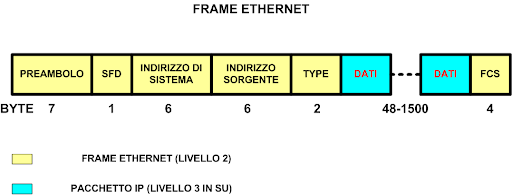
\includegraphics[width=0.9\textwidth]{img/ethernet_frame.png}
\end{center}

\subsubsection{Switch a livello di collegamento}
Gli \textbf{switch} (commutatori) sono i dispositivi centrali nelle LAN moderne . Ricevono frame Ethernet e li inoltrano in modo intelligente verso la loro destinazione. A differenza degli hub (vecchi dispositivi che replicavano i bit su tutte le porte), gli switch sono \textit{trasparenti} (plug-and-play) e operano in modo efficiente .

\begin{itemize}
    \item \textbf{Filtraggio e Inoltro (Filtering/Forwarding):} Gli switch mantengono una \textbf{tabella di commutazione (switch table)} che mappa gli indirizzi MAC alle porte di uscita. Quando un frame arriva :
        \begin{itemize}
            \item Se l'indirizzo MAC di destinazione è associato alla stessa porta da cui il frame è arrivato, lo switch \textbf{filtra} (scarta) il frame.
            \item Se l'indirizzo MAC di destinazione è associato a una porta diversa, lo switch \textbf{inoltra} (forward) il frame solo su quella porta specifica.
            \item Se l'indirizzo MAC di destinazione è \textit{sconosciuto} (non presente in tabella) o è l'indirizzo di broadcast, lo switch effettua un \textbf{flood}, ovvero inoltra il frame su \textit{tutte} le porte, tranne quella da cui è arrivato .
        \end{itemize}
    \item \textbf{Auto-apprendimento (Self-learning):} Gli switch costruiscono la loro tabella di commutazione in modo automatico e dinamico :
        \begin{enumerate}
            \item Per ogni frame ricevuto su una porta, lo switch ispeziona l'indirizzo \textbf{MAC sorgente}.
            \item Registra (o aggiorna) nella sua tabella l'associazione tra quell'indirizzo MAC e la porta da cui è arrivato.
            \item Imposta un timer (TTL) per quella voce; se non riceve più frame da quel MAC per un certo periodo, la voce viene rimossa .
        \end{enumerate}
    \item \textbf{Vantaggi rispetto ai Router:} Gli switch sono più semplici, veloci ed economici. Operano solo fino al livello 2 (non guardano gli header IP) .
    \item \textbf{Svantaggi rispetto ai Router:} Non offrono isolamento tra sottoreti (i broadcast si propagano) e non possono scegliere percorsi ottimali in topologie complesse .
\end{itemize}

\subsubsection{VLAN (Virtual LAN)}
Questo è un concetto fondamentale per le reti aziendali e degli ISP. Una \textbf{VLAN} (LAN Virtuale) permette di configurare un singolo switch fisico come se fosse composto da \textbf{più switch virtuali} e indipendenti .

\textbf{Scopi principali} :
\begin{itemize}
    \item \textbf{Isolamento del traffico:} Gli host su una VLAN (es. "VLAN-Marketing") sono in un dominio broadcast separato e non possono comunicare con host su un'altra VLAN (es. "VLAN-Ingegneria"), anche se fisicamente connessi allo stesso switch .
    \item \textbf{Sicurezza:} Si impedisce agli utenti di una rete di "curiosare" nel traffico di un'altra.
    \item \textbf{Efficienza:} I messaggi broadcast (come le richieste ARP) sono confinati all'interno della propria VLAN e non congestionano l'intera rete .
\end{itemize}

Per far comunicare due VLAN diverse, il traffico \textbf{deve} essere inoltrato attraverso un router (o uno switch di Livello 3).

\textbf{VLAN Trunking (Standard 802.1Q):}
Per estendere le VLAN attraverso più switch fisici, si utilizza un \textbf{collegamento trunk} .
\begin{itemize}
    \item Un collegamento trunk è una porta speciale che può trasportare il traffico di \textit{più} VLAN contemporaneamente .
    \item Per fare ciò, i frame che viaggiano sul trunk vengono "etichettati" (tagged) con uno speciale \textbf{Tag VLAN 802.1Q} .
    \item Questo tag (4 byte) viene inserito nell'header Ethernet e specifica l'ID della VLAN a cui il frame appartiene .
    \item Gli switch usano questo tag per sapere a quale VLAN appartiene il frame quando arriva all'altro capo del trunk .
\end{itemize}

\begin{center}
    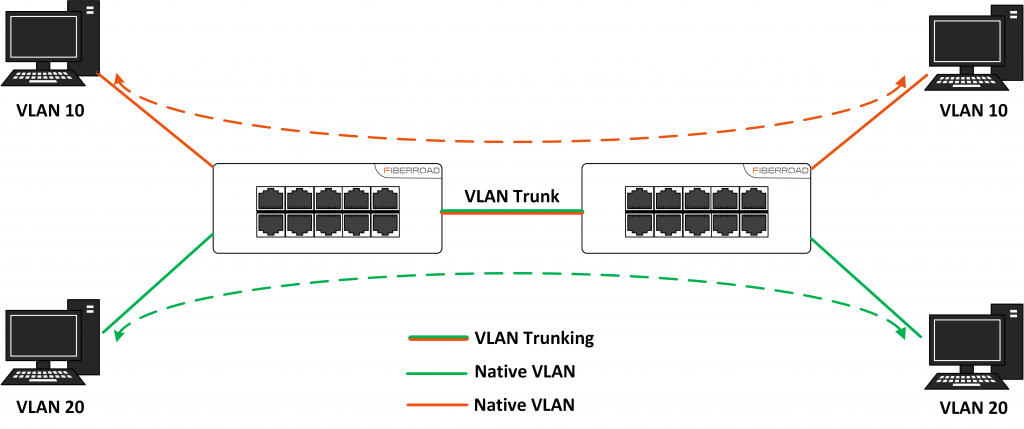
\includegraphics[width=0.8\textwidth]{img/vlan_trunk.png}
\end{center}

\subsection{MPLS (Multiprotocol Label Switching)}
\textbf{MPLS} è una tecnologia del piano dati ad alte prestazioni usata quasi esclusivamente nelle reti dei grandi \textbf{ISP}.

Sebbene MPLS operi "tra" il Livello 2 e il Livello 3, è fondamentale per capire come gli ISP gestiscono il traffico su larga scala. Invece di inoltrare i pacchetti usando le complesse tabelle di inoltro IP (basate sui prefissi di destinazione), i router MPLS usano un meccanismo più semplice e veloce basato su \textbf{etichette (label)} a lunghezza fissa .

\textbf{Funzionamento generale:}
\begin{itemize}
    \item \textbf{Ingresso (LER):} Quando un pacchetto IP entra nella rete dell'ISP, il primo router (Label Edge Router) consulta la sua tabella IP, decide un percorso e "attacca" un'\textbf{intestazione MPLS} (o "shim header") al pacchetto, tra l'header di Livello 2 e quello di Livello 3 .
    \item \textbf{Transito (LSR):} I router interni (Label Switching Routers) non guardano più l'header IP. Leggono solo l'etichetta MPLS, la usano per consultare una tabella MPLS (molto più semplice), "scambiano" (swap) l'etichetta con una nuova etichetta e inoltrano il pacchetto alla porta di uscita successiva .
    \item \textbf{Uscita (LER):} L'ultimo router MPLS rimuove l'etichetta e inoltra il pacchetto IP standard verso la sua destinazione finale.
    \item Il percorso predefinito che i pacchetti seguono è chiamato \textbf{LSP (Label-Switched Path)}.
\end{itemize}

\textbf{Vantaggi Chiave per un ISP:}
\begin{itemize}
    \item \textbf{Ingegneria del Traffico (Traffic Engineering):} Questo è il motivo principale. Gli ISP possono definire LSP espliciti per forzare il traffico a seguire percorsi specifici, bypassando il percorso a costo minimo calcolato da OSPF . Questo è essenziale per bilanciare il carico sulla propria dorsale e ottimizzare l'uso delle risorse di rete.
    \item \textbf{VPN MPLS (BGP/MPLS VPN):} È il meccanismo standard con cui gli ISP offrono servizi \textbf{VPN} ai loro clienti business. MPLS permette di tenere il traffico di clienti diversi (che potrebbero usare gli stessi indirizzi IP privati) completamente isolato mentre viaggia sull'infrastruttura condivisa dell'ISP.
\end{itemize}
